\documentclass[10pt,a4paper]{article}
\usepackage[utf8]{inputenc}
\usepackage{amsmath}
\usepackage{amsfonts}
\usepackage{amssymb}
\usepackage{graphicx}
\usepackage{placeins}

\begin{document}

\section*{Thermodynamics Scratch Sheet}


	\begin{figure}[h]
		\centering
		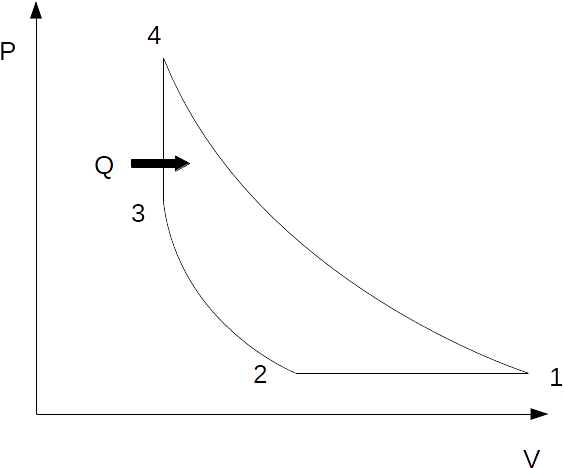
\includegraphics[width=.5\textwidth]{ThermoDiagram.png}
		\caption{PV Diagram of Modern Atkinson Cycle}
		\label{fig:diagram1}
	\end{figure}
	The engine has 6 cylinders and 3000 c.c. total swept volume. The fuel used will be standard octane gasoline. Intake is taken from the ambient atmosphere.\\
	A modern atkinson cycle is chosen in-lieu of the traditional Otto cycle for it's increased ideal efficiency and better mixing properties.\\
	These parameters completely define our thermal cycle. Since the proportion of gasoline is small, and gasoline composed of nonpolar substances, an Ideal Gas model is assumed.
	\subsection*{Initial Constraints}
	Our compression ratio is taken to be 10, a high compression ratio that prevents knocking. \\
	Likewise, a standard air to fuel mixture ratio of 14.7 is chosen.
	\begin{align}
		C_R &= \frac{V_2}{V_3} \\
		M_R &= \frac{m_A}{m_G} = 14.7
	\end{align}
	The volumes are constrained by the total c.c. of the engine. Likewise, it is noted process 3-4 is isochoric.
	\begin{align}
		V_4 &= V_3\\
		\frac{3000\ \text{c.c.}}{6} &= V_1-V_4 
	\end{align}
	Finally, point 1 and point 2 are at ambient pressure $p_{amb}$ and temperature $T_{amb}$.
	\subsection*{Process 2 to 3}
	Using the isentropic equations, $p_3$ is solved for.
	\begin{align}
	\frac{p_3}{p_2} = C_R^{\gamma}\\
	p_3 = p_{amb} C_R^{\gamma}
	\end{align}
	\subsection*{Process 3 to 4}
	The total volume $V_2$ determines the total energy input. By setting up volume mass relations and using the mix ratio, the total mass of the gasoline can be found. This leaves a $V_2$ in the unknowns.
	\begin{align}
	V_G &= m_g R_g \frac{T_2}{p_2} = m_g R_g \frac{T_{amb}}{p_{amb}}\\
	V_A &= m_a R_a \frac{T_{amb}}{p_{amb}}\\
	V_2 &= V_G + V_A = m_G \frac{T_{amb}}{p_{amb}} (R_G + M_R R_A)\\
	m_G &= \frac{V_2 p_{amb}}{T_{amb}(R_G + M_R R_A)}\\
	Q &= m_G H_G
	\end{align}
	Next, using energy conservation, an equation is set up to solve for $p_4$. Since this process is isochoric, W = 0.
	\begin{align}
		\frac{3}{2} p_4 V_4 &= \frac{3}{2} p_3 V_4 + Q
	\end{align}
	\subsection*{Process 4 to 1}
	Finally, isentropic relations are used to create one final equation.
	\begin{align}
		\frac{p_4}{p_{amb}} = \Big( \frac{V_1}{V_4} \Big)^{\gamma}
	\end{align}
	\subsection*{Solving for Unknowns}
	Currently there are 5 unknowns: $V_1\ V_2\ V_3\ V_4\ p_4$ \\
	The 5 equations used to solve them are listed below:
	\begin{align}
	\frac{3000\ \text{c.c.}}{6} &= V_S = V_1-V_4\\	
	C_R &= \frac{V_2}{V_3} \\
	Q &= m_G H_G = \frac{H_G p_{amb} V_2}{T_{amb}(R_G + M_R R_A)} \\
	\frac{3}{2} p_4 V_4 &= \frac{3}{2} p_3 V_4 + Q \\
	\frac{p_4}{p_{amb}} &= \Big( \frac{V_1}{V_4} \Big)^{\gamma}	
	\end{align}
	Plugging in interim constants and replacing $V_3$ with $V_4$.
	\begin{align}
	V_S &= V_1-V_4\\	
	V_2 &= C_R V_4 \\
	Q &= C_1 V_2 \\
	\frac{3}{2} p_4 V_4 &= \frac{3}{2} p_3 V_4 + C_1 V_2 \\
	\frac{p_4}{p_{amb}} &= \Big( \frac{V_1}{V_4} \Big)^{\gamma}	
	\end{align}
	Substituting in $V_2 = C_R V_4$ and $p_3 = p_{amb} C_R^{\gamma}$ to get:
	\begin{align}
		\frac{3}{2} p_4 V_4 &= \frac{3}{2} p_{amb} C_R^{\gamma} V_4 + C_1 C_R V_4 \\
		p_4 &= p_{amb} C_R^{\gamma} + \frac{2}{3} C_1 C_R
	\end{align}
	Substituting in $V_1 = V_S + V_4$:
	\begin{align}
		\Big( \frac{p_4}{p_{amb}} \Big)^{\frac{1}{\gamma}} &= \frac{V_S + V_4}{V_4}\\
		V_4 \bigg( \Big( \frac{p_4}{p_{amb}} \Big)^{\frac{1}{\gamma}} - 1 \bigg) &= V_S \\
		V_4 &= \frac{V_S}{\Bigg( \Big( \frac{p_4}{p_{amb}} \Big)^{\frac{1}{\gamma}} - 1 \Bigg)}
	\end{align}
	Finally from $V_4$ $V_2$ and $V_1$ are derived:
	\begin{align}
		V_2 &= C_R V_4 \\
		V_1 &= V_S + V_4
	\end{align}
	\subsection{Other properties and power calculation}
	First the temperatures and molar amount is found. Then the power is derived from these:
	\begin{align}
		n &= \frac{p_{amb} V_2}{R T_{amb}}\\
		T_4 &= \frac{p_4 V_4}{n R}\\
		T_3 &= \frac{p_3 V_3}{n R}\\
		W_{cyc} &= \frac{3}{2}n R (T_4-T_{amb}) - p_{amb}(V_1-V_2) - \frac{3}{2}n R (T_3-T_{amb})\\
		P &= 6 W_{cyc} \frac{\omega}{2}
	\end{align}
\end{document}